\documentclass[11pt,a4paper]{article}
\usepackage[utf8]{inputenc}
\usepackage[T1]{fontenc}
\usepackage{amsmath}
\usepackage{amsfonts}
\usepackage{amssymb}
\usepackage{graphicx}
\usepackage{float}
\usepackage{cleveref}

\usepackage{enumitem}
%\setlist[itemize]{nosep,left=0pt}
\setlist[itemize]{left=5pt}
\setlist[enumerate]{left=5pt}
\setlist[description]{left=5pt}

%\usepackage{algorithm}
% \usepackage{algpseudocode}
\usepackage[ruled]{algorithm2e}
\usepackage{algcompatible}
\algblockdefx[Hloop]{Hloop}{EndHloop}[1][]{\textbf{hpx::parallel::for$\_$loop} #1}{\textbf{end parallel for}}
\algblockdefx[Func]{Func}{EndFunc}[1][]{\textbf{Function }}{\textbf{end Function}}

\usepackage{listings}

\lstset{language=C++,
 basicstyle=\ttfamily,
 keywordstyle=\color{azure}\ttfamily,
 stringstyle=\color{amaranth}\ttfamily,
 commentstyle=\color{darkgreen}\ttfamily,
 morecomment=[l][\color{magenta}]{\#},
 breaklines=true
}

\usepackage{xcolor}
\definecolor{mygray}{rgb}{0.57, 0.64, 0.69}

\newcommand{\dd}{\mathrm{d}}
\newcommand{\p}{\partial }
\newcommand{\bolds}[1]{\boldsymbol{#1}}
\newcommand{\bfit}[1]{\textit{\textbf{#1}}}

\usepackage[a4paper, total={7.2in, 10in}]{geometry}

\newcommand{\bmatx}[1]{\begin{bmatrix}
    #1
\end{bmatrix}}

\setcounter{section}{0}

\begin{document}

\begin{center} 
\textbf{\Large Final Project} 
\end{center}

In this project, you will develop a numerical method to solve system of first order ordinary differential equations. As an application of developed numerical method, you will solve the one-dimensional partial differential equation (PDE). The task also includes optimization problem to be solved using two different approaches. 

\section{Problem set 1 (20 marks)}
Let $u = u(t) = [u_1(t), u_2(t), ..., u_n(t)]^T$ be a $n\times 1$ vector of functions of time $t$, where $0 \leq t \leq T$. Let $u$ satisfies following:
\begin{equation}\label{eq:ode}
\frac{\dd }{\dd t} u(t) = A u(t) + f(t),
\end{equation}
where $A = [a_{ij}]$ is a $n\times n$ matrix independent of time $t$ and $u$, and $f = f(t) = [f_1(t), f_2(t), ..., f_n(t)]^T$ a $n\times 1$ vector of functions. Above equation satisfies the following initial condition
\begin{equation}\label{eq:odeIC}
u(0) = u^0,
\end{equation}
where $u^0$ is a $n\times 1$ vector of given numbers. 

Let $\Delta t$ is the step size and $t_1 = 0, t_2 = \Delta t, ..., t_{N_t + 1} = N_t \Delta t$ are the discrete times, $N_t$ being the number of steps. 

\begin{itemize}
\item[(i)] \bfit{Implement} {\it forward Euler} method to solve \eqref{eq:ode} for $u(t_1), u(t_2), ..., u(t_{N_t + 1})$.
\item[(ii)] \bfit{Implement} {\it backward Euler} method to solve \eqref{eq:ode} for $u(t_1), u(t_2), ..., u(t_{N_t + 1})$.
\item[(iii)] \bfit{Test} your implementation by comparing your results for the following specific problem with $n=4$, $T = 1$, $\Delta t = 10^{-5}$, $f(t) = [0, 0, 0, 0]^T$, $u^0 = [1, 0, 0, 0]^T$, and the matrix $A$ given by
\begin{align}
A = \bmatx{-2 & 1 & 0 & 0 \\ 1 & -2 & 1 & 0 \\ 0 & 1 & -2 & 1 \\ 0 & 1 & -1 & 0 }.
\end{align}
\bfit{Compare} your results from both the {\it forward Euler} and {\it backward Euler} with solution $u(T)$ at final time $T$ given by
\begin{equation}
u(T) = [0.2165, 0.1931, 0.1138, 0.1138]^T .
\end{equation}
\item[(iv)] \bfit{Verify} that for large $T$, say $T = 1000$, and $\Delta t = T/10^6$, $u(T)$ is very small (of the order of $10^{-87}$). This is due to the fact that the problem is dissipative. 
\item[(v)] Take $T = 10$ and different $\Delta t = T/2^k$, $k=1,2,3,...,10$.  \bfit{Provide} table of $max(u(T))$, i.e., maximum of four-element vector $u(T)$, for different $k$ (or equivalently different $\Delta t$). 

\noindent\textit{Remark 1.} \bfit{Note} that {\it forward Euler} is unstable for large $\Delta t$. Specifically, it is unstable when $\Delta t$ is such that $\rho(I + \Delta t A) > 1$, where $I$ is the identify matrix, $A$ is the matrix in ODE, $\Delta t$ is the size of time step, and $\rho(A)$ is the spectral radius of matrix $A$. Spectral radius can be computed by first computing the eigenvalues of $A$, then taking the absolute of the eigenvalues, and finally picking the maximum of absolute of eigenvalues. In Matlab you can do this as follows:
\begin{equation}
rho = max (abs(eig(I + \Delta t A))) .
\end{equation}

For a simple ODE $\dd v / \dd t = -\lambda v$ with a positive number $\lambda$,  {\it forward Euler} is unstable if $|1 - \Delta t \lambda | > 1$ and stable if $\Delta t$ is such that $|1 - \Delta t \lambda | \leq 1$. Thus, {\it forward Euler} is stable as long as $\Delta t \leq 2/\lambda$. As you can see, when $\lambda$ is large, one needs to have small $\Delta t$ to keep the {\it forward Euler} stable. On the other hand, {\it backward Euler} is stable as long as $\frac{1}{|1 + \Delta t \lambda|} \leq 1$ which is satisfied for any positive $\Delta t$, i.e., for any $\Delta t$, {\it backward Euler} is stable. In certain situations {\it backward Euler} can compute solutions faster by taking large $\Delta t$.
\end{itemize}

\section{Problem set 2 (35 marks)}
Consider a composite bar in Figure \ref{fig:bar} of length $L$. We are interested in modeling temperature in this bar as a function of position on the bar and time. Let $h = h(t, x)$ be the temperature in bar at point $x$, $0\leq x \leq L$, and time $t$, $0 \leq t \leq T$. The left end is at $x=0$ and the right end is at $x=L = L_1 + L_{12}+L_2$.

The temperature field $h$ satisfies the following one-dimensional heat (or diffusion) partial differential equation, for all $0 \leq t \leq T$ and $0\leq x \leq L$,
\begin{equation}\label{eq:pde}
\frac{\p}{\p t} h(t, x) = k(x) \frac{\p^2 }{\p x^2} h(t, x) + q_{ext}(t, x),
\end{equation}
where $\frac{\p}{\p t} h(t, x)$ is the partial derivative of $h$ with respect to $t$, similarly $\frac{\p}{\p x} h(t, x)$ is the partial derivative with respect to $x$, $k = k(x)$ is the thermal conductivity coefficient as a function of $x$, $q_{ext} = q_{ext}(t, x)$ external source. 

Because the bar is composite, we consider thermal conductivity $k$ as a function of $x$. We consider $k$ as a following function (notice how this function is related to bar in Figure \ref{fig:bar})
\begin{align}\label{eq:cond}
k(x) = \begin{cases}
k_1, & \qquad \text{if } x \leq L_1, \\
k_2, & \qquad \text{if } x \geq L_1+L_{12}, \\
k_1 + (k_2 - k_1)\frac{(x - L_1)}{L_{12} }, &\qquad \text{otherwise}.
\end{cases}
\end{align}
In the above, $k$ goes to $k_1$ at $x \leq L_1$ to $k_2$ at $x \geq L_1+L_{12}$ linearly over the length $L_{12}$. We fix $L_{12} = 0.1$ and keep $L_1$ and $L_2$ as flexible. Note that since $L_1 + L_2 + L_{12} = L$, if $L$ and $L_{12}$ are fixed, only one of the two, $L_1$ or $L_2$, will be independent. 

We also consider the following external source
\begin{equation}\label{eq:qext}
q_{ext}(t, x) = \alpha \exp(-\beta x) \sin(\theta x),
\end{equation}
where $\alpha = 200, \beta = 2, \theta = 20$.

Since we are dealing with the partial differential equation that includes the first order time derivative and the second order space derivative, we need one initial condition and two boundary conditions. We consider the following initial condition
\begin{equation}\label{eq:pdeIC}
h(0, x) = 0, \qquad 0 \leq x \leq L
\end{equation}
and boundary conditions
\begin{equation}
h(t, 0) = 100, \qquad \frac{\p h(t, L)}{\p x} = 0, \qquad 0 < t \leq T.
\end{equation}
We basically fixed the temperature at the left-end of the bar to $100$ and the heat flux at the right-end to zero.

\begin{figure}
\centering
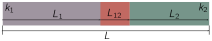
\includegraphics[width=0.7\linewidth]{bar}
\caption{Composite bar with different material properties. In orange region, transition of conductivity $k_1$ to $k_2$ takes place linearly.}
\label{fig:bar}
\end{figure}

\vspace{10pt}
\noindent\textit{Parameters.} Let $T = 1$, $L = 1$, $N_t = 1000$, $\Delta t = T/ N_t$, $N_x = 1000$, $\Delta x = L /N_x$, $k_1 = 10$, $k_2 = 0.1$, $L_{12} = 0.1$, $L_1 = 0.7$, $L_2 = 0.2$, $\alpha = 200$, $\beta = 2$, $\theta = 20$. Functions $k$ and $q_{ext}$ are given in \eqref{eq:cond} and \eqref{eq:qext}, respectively.  

\subsection{Numerical method to solve the heat equation}
Let $\Delta x$ be the mesh size such that $x_1 = 0, x_2 = \Delta x, x_3 = 2\Delta x, ..., x_{N_x + 1} = N_x \Delta x$ are the discrete points on the bar. Let $H_i = H_i(t) = h(t, x_i)$ is the temperature at point $x_i$ on the bar as a function of time $t$. 

\begin{itemize}
\item[(i)] \bfit{Obtain} the system of the first order ODE from \eqref{eq:pde} (through approximation of $\p^2 h(t, x_i)/ \p x^2$) of the form:
\begin{equation}\label{eq:pdeDisc}
\frac{\dd}{\dd t} H(t) = A H(t) + Q_{ext} (t),
\end{equation}
where $H(t) = [H_2(t), H_3(t), ..., H_{N_x + 1}(t)]^T$ is the $N_x \times 1$ vector of function of temperature at points $x_2, x_3, ..., x_{N_x + 1}$, $A$ is the $N_x \times N_x$ matrix, $Q_{ext} = Q_{ext}(t)$ is the vector of function. \bfit{Provide} the structure of matrix $A$ and $Q_{ext}$ for general $\Delta x$.  Note that in above I have used $\dd H_(t) / \dd t$ because vector function $H$ is just a function of $t$.

\bfit{Note} that matrix $A$ will be familiar to you. However, in this problem because of the boundary condition $\p h(t, L) / \p x = 0$, the matrix $A$ will be slightly different. Follow the hints.  

\item[(ii)] Consider discrete times: $t_1 = 0, t_2 = \Delta t, t_3 = 2\Delta t, ..., t_{N_t + 1} = N_t \Delta t$. Using the parameters specified in the previous section and the method developed in {\bf Problem set 1}, numerically \bfit{solve} for $H(t_k)$ for $k=2, 3, ..., N_t + 1$. Note that from the initial condition \eqref{eq:pdeIC}, we know $H(t_1)$. \bfit{Use} {\it backward Euler} method. 

\bfit{Plot} (on the same plot using `hold on') $H(t_k)$, $k=201, 401, 601, 801, 1001$, as a function of $x$. For a given $t$, $H(t)$ is a vector with each element of the vector corresponding to different points $x$ on the bar. So you can plot the points $x_i$ on bar in the x-axis and corresponding temperature $H_i(t)$ in the y-axis.

\item[(iii)] \bfit{Try} different $\Delta t$ staring with a large to a very small and \bfit{report} the $\Delta t$ such that {it forward Euler} method is stable for the above problem. For this problem, let $T = 0.001$. You can try $N_t = 1000, 5000, 10000, ...$ and so on until $H(T)$ (solution at last time) is reasonable. (Reasonable means that the vector $H(T)$ has maximum value of $100$ (boundary condition temperature) and minimum value $0$.) This exercise shows that even for simple problem like above, \textit{forward} Euler is not a good choice as it requires very small $\Delta t$ to have stable solution. I recommend not storing the whole solution vector $H(t_1), H(t_2), ..., H(t_{N_t + 1})$ because if $N_t$ is very large, you will be storing a lot of data. Just store the solution $H(t_{N_t + 1})$ at final time step.
\end{itemize}
 
\section{Problem set 3 (35 marks)}
{\color{red} To be done independently. There will be a high penalty if we find any sign of collaboration on this problem set.}

\noindent Notice that the composite bar consists of two materials. One of the material has a very high thermal conductivity whereas the other has a very low conductivity. The material with $k_2 = 0.1$ can be thought of as thermal insulator. Goal of this problem is to find the optimal length $L_2$ of the second material so that the temperature at the right-end of the bar at final time $T = 1$, i.e., $h(T, L)$, is about $50$. 

There are two ways to find the optimal $L_2$ such that $h(T, L) = 50$. But, before we perform this calculation, we change the partial differential equation slightly to also include the {\it convection} effect:

\begin{equation}\label{eq:pde2}
\frac{\p}{\p t} h(t, x) = k(x) \frac{\p^2 }{\p x^2} h(t, x) - c \frac{\p }{\p x} h(t, x) + q_{ext}(t, x),
\end{equation}
where the new term $c$ is the convection velocity. We let $c = 0.001$. 

\begin{itemize}
\item[(i)] As in the problem 2, discretize the bar with discrete points $x_1 = 0, x_2 = \Delta x, ..., x_{N_x + 1} = N_x \Delta x$. \bfit{Convert} \eqref{eq:pde2} into the system of ordinary differential equation of type (through approximation of $\p^2 h(t, x_i)/ \p x^2$ and $\p h(t, x_i)/\p x$):
\begin{equation}\label{eq:pdeDisc2}
\frac{\dd }{\dd t} H(t) = A H(t) + Q_{ext} (t).
\end{equation}
In this case, \bfit{what} is the matrix $A$? Use the {\it forward difference} to approximate $\p h(t, x_i)/\p x$. 

\item[(ii)] {\bf Method 1: Regression method.} Consider $L_2 = 0.02, 0.02+\Delta L_2, 0.02 + 2\Delta L_2, ..., 0.02 + 15\Delta L_2$ with $\Delta L_2 = 0.05$. For each value of parameter $L_2$, \bfit{solve} the \eqref{eq:pdeDisc2} and obtain $h(T, L)$ (temperature at the final time and at the right-end of the bar, $h(t, x)$ with $t = T$ and $x = L$). Keep all parameters except $L_2$ same as described in Section 2. Also fix $c = 0.001$.

{\bf Step 1: } \bfit{Provide} a table of values where the first column is $L_2$ and the second column is $h(T, L)$. 

{\bf Step 2: } Using the above table as data ($L_2$ is the independent variable and $h(T, L)$ is the dependent variable on $L_2$), \bfit{explain} what type of {\it curve fitting} (regression or interpolation) is appropriate.

{\bf Step 3: } \bfit{Perform} curve fitting of the data in the table by choosing sufficiently high order polynomial function.

{\bf Step 4: } From the curve-fitting, \bfit{find} the independent variable $L_2$ such that $h(T, L) = 50$. 

{\bf Step 5: } Use $L_2$ you obtained in step 4 and solve the problem \eqref{eq:pdeDisc2}. \bfit{How} much does the model solution $h(T, L)$ differ from the target value of $50$ for the selected $L_2$?

\item[(iii)] {\bf Method 2: Optimization.} Write a code that takes $L_2$ as input and returns $h(T, L)$ by solving \eqref{eq:pdeDisc2}. Let $f = h(T, L)$, and since $f$ depends on $L_2$, let $f = f(L_2)$. So, your code should compute $f(L_2)$ for a given $L_2$. 

Define the {\it squared-error} cost function for the optimization by
\begin{equation}
J = J(L_2) = (f(L_2) - 50)^2.
\end{equation}
With the initial guess of $L_2 = 0.07$, and the lower and upper bounds $0.05$ and $0.2$ on $L_2$, respectively, \bfit{apply} `fmincon' to find the optimal $L_2$. \bfit{Report} the optimal $L_2$ and the corresponding value of $h(T, L)$. 

\end{itemize}


\section{Guidelines for preparing project report} 
Reports carry 10 marks. Your report will have four sections in the following order:
\begin{itemize}
\item[1.] In this section, you will discuss the physical significance and application of the problem and general method, and what you have learned in doing this project.
\item[2.] Answers to all the problem sets 1, 2, and 3. You must prepare this report such that it is self-contained. 
\item[3.] In this section, discuss the role of different members in completing this project. Provide some specific details of individual contributions just so we know everyone in the group worked sincerely. 
\item[4.] Attach your codes as a supplement to this report.
\end{itemize}

{\color{red} {\bf Note.} For problem set 3, collaboration is strictly not allowed. If we find any sign of collaboration on problem set 3, there will be heavy penalty.

The codes for problem set 2 must not be generalized to include the components of problem set 3. Basically, work on the problem set 3 separately from the other problem sets. }


\section{Grading for the final project}
Because the problem set 3 really shows whether you have grasped the numerical method in problem set 1 and 2, we will assign following conditional marks:

Suppose you get marks $a$, where $0 \leq a \leq 35$, on problem set 3. We will subtract $min\{35 - a, 10\}$ marks from the problem set 1 and $\min\{35 - a, 20\}$ from the problem set 2. 

Example: if $a = 20$, then you will loose $10$ and $15$ marks from problem sets 1 and 2. If $ a = 10$, then you will loose $10$ and $20$ from problem sets 1 and 2.

\section{Some hints}
This project builds on ideas you have already mastered in previous projects and assignments. There is just one part where you will require some help. 

In developing a numerical method for PDE
\begin{equation}\label{eq:pdeHelp}
\frac{\p}{\p t} h(t, x) = k(x) \frac{\p^2 }{\p x^2} h(t, x) + q_{ext}(t, x),
\end{equation}
you will need to approximate the term  $\frac{\p^2 }{\p x^2} h(t, x_i)$ at some discrete point $x_i$ for given $t$. 

\paragraph{Definition of partial derivatives}
We note how partial derivatives are defined to construct an approximation. We have:
\begin{align}
\frac{\p}{\p t} h(t, x) &= \lim_{a \to 0} \frac{h(t + a, x) - h(t,x)}{a} = \lim_{a \to 0} \frac{h(t, x) - h(t-a,x)}{a} = \lim_{a \to 0} \frac{h(t + a, x) - h(t-a,x)}{2a}, \notag\\
\frac{\p}{\p x} h(t, x) &= \lim_{a \to 0} \frac{h(t , x+a) - h(t,x)}{a} = \lim_{a \to 0} \frac{h(t, x) - h(t, x - a)}{a} = \lim_{a \to 0} \frac{h(t, x+a) - h(t,x-a)}{2a}
\end{align}
and
\begin{align}
\frac{\p^2}{\p x^2} h(t, x) &= \lim_{a \to 0} \frac{\frac{\p}{\p x} h(t, x+a) - \frac{\p}{\p x} h(t, x)}{a} = \lim_{a \to 0} \frac{\frac{\p}{\p x} h(t, x) - \frac{\p}{\p x} h(t, x-a)}{a} \notag \\
&= \lim_{a \to 0} \frac{\frac{\p}{\p x} h(t, x+a) - \frac{\p}{\p x} h(t, x-a)}{2a}.
\end{align}
For the exterior points $x = 0$ and $x=L$ (and also $t=0$ and $t=T$), one of these formula will not be valid if $x-a$ or $x+a$ is outside the domain of function $[0,L]$ (similarly, if $t-a$ or $t+a$ is outside $[0,T]$). The idea is that to get partial derivative with respect to one variable, we fix all other variables and change only one variable for which partial derivative is computed.

\paragraph{Approximation of partial derivatives}
For interior point $x_i$, i.e., $i=2, 3, ..., N_x$ (except $i=1$ and $i=N_x + 1$), you can use the central-difference formula as follows:
\begin{equation}
\frac{\p^2 }{\p x^2} h(t, x_i) \approx \frac{h(t, x_{i+1}) - 2h(t, x_i) + h(t, x_{i-1})}{\Delta x^2},
\end{equation}
where $\Delta x$ is the spacing between discrete points. For the exterior point $x_1 = 0$, you do not need to approximate this term, as $h(t, x_1)$ is given by the boundary condition. 

For the remaining exterior point $x_{N_x + 1} = L$, we need to be little careful as we are also given the boundary condition: 
\begin{equation}
\frac{\p }{\p x} h(t, x_{N_x + 1}) = \frac{\p }{\p x} h(t, L) = 0.
\end{equation}
We consider the following approximation of $\frac{\p^2 }{\p x^2} h(t, x_{N_x + 1})$:
\begin{align}
\frac{\p^2 }{\p x^2} h(t, x_{N_x + 1}) &\approx \frac{\frac{\p }{\p x} h(t, x_{N_x + 1}) - \frac{\p }{\p x} h(t, x_{N_x})}{\Delta x} \notag \\
&= \frac{ - \frac{\p }{\p x} h(t, x_{N_x})}{\Delta x} \notag \\
&\approx \frac{-1}{\Delta x} \left[ \frac{h(t, x_{N_x + 1}) - h(t, x_{N_x})}{\Delta x} \right],
\end{align}
where we used the boundary condition $\frac{\p }{\p x} h(t, x_{N_x + 1}) = 0$ in the second last step, and used the forward difference formula to approximation $ \frac{\p }{\p x} h(t, x_{N_x})$. Above provides the approximation of $\frac{\p^2 }{\p x^2} h(t, x_{N_x + 1})$. 

Similarly, for the problem set 3, you may approximate the $\frac{\p }{\p x} h(t, x_i)$ at any interior points using the forward difference approximation
\begin{equation}
\frac{\p }{\p x} h(t, x_i) \approx \frac{h(t, x_{i+1}) - h(t, x_i)}{\Delta x}.
\end{equation}
Again, you do not need to worry about the exterior point $x_1 = 0$. For the other exterior point $x_{N_x + 1} = L$, you do not need to do anything as the boundary condition sets $\frac{\p }{\p x} h(t, x_{N_x + 1}) = 0$. 


\end{document}